\documentclass[10pt,twocolumn,letterpaper]{article}

\usepackage{cvpr}
\usepackage{times}
\usepackage{epsfig}
\usepackage{graphicx}
\usepackage{amsmath}
\usepackage{amssymb}
\usepackage[table,xcdraw]{xcolor}
\usepackage{bbm}
\usepackage{subfig}
\usepackage{caption}
\usepackage{subcaption}
\usepackage{enumitem}

% Include other packages here, before hyperref.

% If you comment hyperref and then uncomment it, you should delete
% egpaper.aux before re-running latex.  (Or just hit 'q' on the first latex
% run, let it finish, and you should be clear).
\usepackage[pagebackref=true,breaklinks=true,letterpaper=true,colorlinks,bookmarks=false]{hyperref}

\cvprfinalcopy % *** Uncomment this line for the final submission

\def\cvprPaperID{****} % *** Enter the CVPR Paper ID here
\def\httilde{\mbox{\tt\raisebox{-.5ex}{\symbol{126}}}}

% Pages are numbered in submission mode, and unnumbered in camera-ready
% \ifcvprfinal\pagestyle{empty}\fi
\begin{document}

%%%%%%%%% TITLE
\title{Real-Time Flying Object Detection}

\author{Dillon Reis*, Jordan Kupec*, Jacqueline Hong*, Ahmad Daoudi*\\
Georgia Institute of Technology\\
{\tt\small dreis7@gatech.edu, jkupec3@gatech.edu, jhong356@gatech.edu, adaoudi3@gatech.edu}
% For a paper whose authors are all at the same institution,
% omit the following lines up until the closing ``}''.
% Additional authors and addresses can be added with ``\and'',
% just like the second author.
% To save space, use either the email address or home page, not both
}

\maketitle
%\thispagestyle{empty}

%%%%%%%%% ABSTRACT
\begin{abstract}
   This project presents a generalized model for real-time detection of flying objects that is ready for immediate implementation, transfer learning, or further research with potential uses by remote digital airport towers, unmanned aerial vehicles (UAVs), or any surveillance systems incorporating optical data. Real-time object detection remains challenging due to large variance object spatial sizes/aspect ratios during inference, object rate of speed, occlusion ,and clustered backgrounds. To address some of the presented challenges while simultaneously maximizing performance, we utilize the current state of the art single-shot detector, YOLOv8, in an attempt to find the best trade-off between inference speed and mAP. While YOLOv8 is being regarded as the new state-of-the-art \cite{state-of-the-art}, an official paper has not been provided. Thus, we provide an in depth explanation of the new architecture and functionality that YOLOv8 has adapted. RESULTS TBD
\end{abstract}

%%%%%%%%% BODY TEXT
\section{Introduction/Background/Motivation}
Numerous recent events have demonstrated the malicious use of drones. Over the past few months, there have been reports of assassination attempts via drones with small explosive payloads \cite{SuicideDrone}, delivering drugs into state prisons \cite{PrisonDrugs}, and surveillance of U.S. Border Patrol by smugglers \cite{BorderPatrol}. While research indicates that drone usage is expected to increase exponentially \cite{DroneMarket}, detection technology have yet to provide reliable and accurate results. Drones and mini UAVs present a stealth capability and can avoid detection by most modern radar systems due to their small electromagnetic signature. They are also small, highly maneuverable, and omit low levels of noise. This, along with the ease of access provides a natural incentive for drones to remain an integral part of modern warfare and illegal activities. While methods such as radio and acoustic detection have been proposed as solutions, they are currently known to be inaccurate \cite{Drone-Detection-Using-YOLOv5}. This motivates the integration of a visual detector in any such detection system. To lay out the process of tackling this problem, we will focus on the real-world use case of drone surveillance conducted by smugglers at the U.S. border.

After an encounter with about 30 migrants illegally crossing the border into the U.S., a subsequent investigation led to the discovery of footage recorded by the smugglers of the entire encounter. The U.S. Border Patrol already has digital towers that utilize object detection in order to monitor people and motor vehicles \cite{BorderDetection}, but to the best of our knowledge, they do not detect drones. Their technology primarily focuses on finding migrants but lacks the ability to detect their drones. The surrounding conditions of the border consist of large spans of isolated land and compacted collections of plants which is known to cause issues for object detection algorithms \cite{BorderDigitalTowers}, making the landscape and background a challenge for drone detection. Additionally, if the object is far away, not only will it be difficult to detect it, but it will also be harder to correctly classify it as the object will convey less signal to the model. Previous research and projects on flying object detection have a predominant focus on UAVs, specifically Drone-vs-Bird. This is not a proper reflection of real-world conditions, as there are many different varieties of flying objects. We plan to integrate more classes such as specific military and commercial aircraft in our training (citation) to let the model see more variance of flying objects and to better understand important features that make up these objects, leading to a more generalized real-time flying object detection model. We then transfer learn these weights on a data set more representative of real world scenarios with high variance in spatial sizes and backgrounds to train our final model.  

The primary objective of this project is to provide generalized real-time flying object detection model that is ready to use ``out of the box'' for immediate implementation, transfer learning, or further research. We define a generalized model as one that has good detection and classification performance at higher resolutions while maintaining a reasonable frame rate (1080p : 30-60 frames per second). To maximize our models performance, we use the latest state-of-the-art single-shot detector, YOLOv8. Currently, single-stage detectors are the de-facto architecture choice for fast inference speeds. This choice comes at the expense of exchanging the higher accuracy you would typically expect from a two-state detector. While YOLOv8 is being regarded as the new state-of-the-art \cite{state-of-the-art}, an official paper has yet to be released. This motivates our secondary objective, which is to explain the new architecture and functionality that YOLOv8 has adapted. 

Real-time object detection remains challenging due to variances in object spatial sizes and aspect ratios, inference speed, and noise. This is especially true for our use case, as flying objects can change location, scale, rotation, and trajectory very quickly. This conveys the necessity for fast inference speed and thorough model evaluation between low-variance classes, object sizes, rotations, backgrounds, and aspect ratios.

Our initial model is trained on a dataset \cite{InitialDataset} comprised of 15,064 images of various flying objects with an 80\% train and 20\% validation split. Each image is labeled with the class number of the object and the coordinates of the edges of the associated bounding box. An image may have more than one object and class, sitting at an average of 1.6 annotated objects per image and a total of 24,769 annotations across all images. The median image ratio is 416x416. The images were pre-processed with auto-orientation, but there were no augmentations applied. The dataset represents a long-tailed distribution with the drone (25.2\% of objects), bird (25\%), p-airplane (7.9\%), and c-helicopter (6.3\%) classes taking up the majority of the dataset (64.4\%), suffering from a class imbalance. Published on Roboflow with an unnamed author, this dataset was generated in 2022, having been downloaded only 15 times.

In addition, we utilized a second data set \cite{TransferDataset} to apply transfer learning. With a focus on the challenges we laid out, this second dataset is of flying objects at a noticeably farther distance than our initial dataset. It consists of 11,998 images, where the average image size is 0.33 mp with a median image ratio of 640x512. The images are separated into a 90\% train and 10\% validation split. An image may contain more than one object and class, however, it has an average of one object per image, reaching a total count of 12,410 annotated objects. With only four different objects, each class is well represented: drones take up 38.8\% of the annotated objects, 21.2\% helicopters, 20.4\% airplanes, and 19.6\% birds. Although Roboflow reports a bird class, the images that contain birds are not labeled and are not included as a class in the transfer model. This dataset was published on Roboflow in 2022 by Ahmed Mohsen, having only 5 downloads by the time of this paper.
%-------------------------------------------------------------------------
%------------------------------------------------------------------------
\section{Approach}

We chose the YOLOv8 architecture under the assumption that it would provide us the highest probability of success given the task. YoloV8 is 
assumed to be the new state-of-the-art due to its higher mAPs and lower inference speed on the COCO dataset(NEED YOLO COMPARISON GRAPHS COCO). However, an official paper has 
yet to be released. It also specifically performs better at detecting aerial objects \ref{fig:YOLOv8_average_mAP_against_cats}, which is the scope of this project. We implement the code
from Ultralytics repository. We decide to implement transfer learning and initialize our models with pre-trained weights to then begin training on the 
custom data set. These weights are from a model trained on the COCO dataset \cite{coco}. Due to only having access to a single NVIDIA RTX 3080 and 3070, 
a greedy model selection/hyper-parameter tuning approach was chosen. We first train a version of the small, medium, and large versions of the 
model with default hyper-parameters for 100 epochs. Then, we decide which model is optimal for our use case given the trade off between inference 
speed and mAP-50-95 on the validation set. After the model size is selected, a greedy hyper-parameter search is conducted with 10 epochs per each 
set of hyper-parameters. The model with the optimal hyper-parameters trains for 163 epochs to generate the initial model. After this model learns abstract feature representations for a wide-array of flying objects, we then transfer learn these weights on a much simpler data set that represents our primary objective and the real world (REEEEF) to generate the final model. This data set contains 3 classes: helicopter, plane, and drone, with very high variance in object spatial sizes. For evaluation, we are only interested in maP50-95 and inference speed.
Mean Average Precision (mAP) is a commonly used evaluation metric for object detection that combines precision, recall, IOU, and AP. The curve we obtain is commonly called the precision-recall curve. Average Precision is therefore defined as the area underneath this curve. A higher AP score indicates better performance since it means the model is accurately detecting more objects in an image while minimizing false positives.
For each class, we divide the recall values into 11 points ranging from 0.5 to 0.95 with step-size 0.05 plot that against maximum precision from that recall value upward. We obtain mAP by averaging over each classes AP \ref{mAP}\\ 

\begin{align}\label{mAP}
AP=\dfrac{1}{9}\sum_{IoU\in{0.5,...0.95}}AP_r \\*
=\dfrac{1}{9}\sum_{r\in{0.5,...0.95}}p_{interp}{r}
\end{align}
where:
\begin{equation*}
p_{interp}({r}) = \max_{\widetilde{r}\geq{r}} p(\widetilde{r})
\end{equation*}
Due to the large class imbalance, poor performance on the validation set was anticipated on the minority classes. However, this was not observed\ref{fig:confusion_matrix}.

\subsection{Initial Model Choice and Evaluation}

We evaluate small, medium, and large versions of the models to determine an optimal trade off between inference speed and mAP50-95 to then optimize the hyper-parameters. The small, medium, and large models have (11151080, 25879480, \& 43660680) parameters and (225,295, \& 365) layers respectively. After training the models we see there is a noticeable increase in mAP50-95 between small and medium models (0.05), but not much delta between medium and large (0.002). We also see that small, medium, and large infer at 4.1,5.7, and 9.3 milliseconds respectively on the validation set. However, our original goal is to reach an average inference speed between 30 to 60 frames for 1080p. When testing the medium size model on multiple 1080p HD videos, we observe an average total speed (pre-proccess speed(0.5ms) + inference speed(17.25ms) + post-process speed(2ms)) of 19.75 ms (50 frames per second), which aligns with our primary objective. This leads to our selection of the medium size model to begin tuning hyper-parameters.

Due to a lack of computational resources, we evaluate only 10 epochs for each small set of hyper-parameters as an indicator for the potential performance of additional epochs. We observe that this assumption is correct, as training with the optimal set of hyper parameters achieves better performance at epoch 100 compared to default hyper-parameters (0.027)\ref{fig:YOLOv8_mAP50-95_val} We choose the best hyper-parameters based on validation mAP50-95 as batch size of 16, stochastic gradient descent (SGD) as the optimizer, momentum of 0.937, weight decay of 0.01, classification loss weight $\lambda_{cls}$ = 1, box loss weight $\lambda_{box}$ = 5.5, and distribution focal loss weight $\lambda_{dfl}$ = 2.5. After training for 163 epochs we achieve an mAP50-95 of 0.685 and recall of 0.792.

\subsection{Loss Function and Update Rule}
The generalized loss function and weight update procedure can be defined as follows: 
\begin{equation}\label{Generalized Loss}
\mathcal{L}(\theta) = \dfrac{\lambda_{box}}{N_{pos}}\mathcal{L}_{box}(\theta) + \dfrac{\lambda_{cls}}{N_{pos}}\mathcal{L}_{cls}(\theta) + \dfrac{\lambda_{dfl}}{N_{pos}}\mathcal{L}_{dfl}(\theta) + \phi\Vert \theta \Vert_2^2
\end{equation}    
\begin{equation}\label{Velocity}
V^t = \beta V^{t-1} + \nabla_{\theta}\mathcal{L}(\theta^{t-1})
\end{equation}    
\begin{equation}\label{Weight Update}
\theta^{t} = \theta^{t-1} - \eta V^{t}
\end{equation}

Where \ref{Generalized Loss} is the generalized loss function incorporating the individual loss weights and a regularization term with weight decay $\phi$, \ref{Velocity} is the velocity term with momentum $\beta$, and \ref{Weight Update} which is the weight update rule and $\eta$ is the learning rate. The specific YoloV8 loss function can be defined as:
\begin{multline}
\mathcal{L} = \dfrac{\lambda_{box}}{N_{pos}}\sum_{x,y}\mathbbm{1}_{c^*_{x,y}}\big[1 - q_{x,y} + \dfrac{\Vert b_{x,y} - \hat{b}_{x,y} \Vert_2^2}{\rho^2} + \alpha_{x,y}\nu_{x,y}\big] \\  + \dfrac{\lambda_{cls}}{N_{pos}}\sum_{x,y}\sum_{c\in classes}y_clog(\hat{y}_c) + (1 - y_c)log(1 - \hat{y}_c) \\
+ \dfrac{\lambda_{dfl}}{N_{pos}}\sum_{x,y}\mathbbm{1}_{c^*_{x,y}}\Big[-(q_{(x,y)+1} - q_{x,y})log(\hat{q}_{x,y}) \\
+ (q_{x,y} - q_{(x,y)-1})log(\hat{q}_{(x,y)+1})\Big]
\end{multline}

where:
\begin{equation*}\label{IoU}
q_{x,y} = IoU_{x,y} = \dfrac{\hat{\beta}_{x,y}\displaystyle \cap\beta_{x,y}}{\hat{\beta}_{x,y}\displaystyle \cup\beta_{x,y}}
\end{equation*}
\begin{equation*}\label{v}
\nu_{x,y} = \dfrac{4}{\pi^2}(arctan(\dfrac{w_{x,y}}{h_{x,y}}) - arctan(\dfrac{\hat{w}_{x,y}}{\hat{h}_{x,y}}))^2
\end{equation*}
\begin{equation*}\label{a}
\alpha_{x,y} = \dfrac{\nu}{1 - q_{x,y}}
\end{equation*}
\begin{equation*}\label{y_hat}
\hat{y}_c = \sigma({\cdot})
\end{equation*}
\begin{equation*}\label{q_hat}
\hat{q}_{x,y} = softmax({\cdot})
\end{equation*}
    
    
and:
\begin{itemize}
\item $N_{pos}$ is the total number of cells containing an object.
\item $\mathbbm{1}_{c^*_{x,y}}$ is an indicator function for the cells containing an object. 
\item $\beta_{x,y}$ is a tuple that represents the ground truth bounding box consisting of ($x_{coord}$,$y_{coord}$,width,height).
\item $\hat{\beta_{x,y}}$ is the respective cell predicted box.
\item $b_{x,y}$ is a tuple that represents the central point of ground truth bounding box.
\item $y_c$ is the ground truth label for class c (not grid cell c) for each individual grid cell (x,y) in the input, regardless if an object is present
\item $q_{(x,y)+/- 1}$ are the nearest predicted boxes IoUs (left and right) $\in c^*_{x,y}$
\item $w_{x,y}$ and $h_{x,y}$ are the respective boxes width and height.
\item $\rho$ is the diagonal length of the smallest enclosing box covering the predicted and ground truth boxes.
\end{itemize}

Each cell then determines its best candidate for predicting the bounding box of the object. This loss function includes the CIoU (complete IoU) loss proposed by Zheng et al.\cite{CIoU} as the box loss, the standard binary cross entropy for multi-label classification as the classification loss (allowing each cell to predict more than 1 class), and the distribution focal loss proposed by Li et al.\cite{GFL} as the 3rd term.
    
\begin{figure*}[h]
    \centering
    \subfloat[\centering Confusion matrix for all classes \label{fig:confusion_matrix}]{{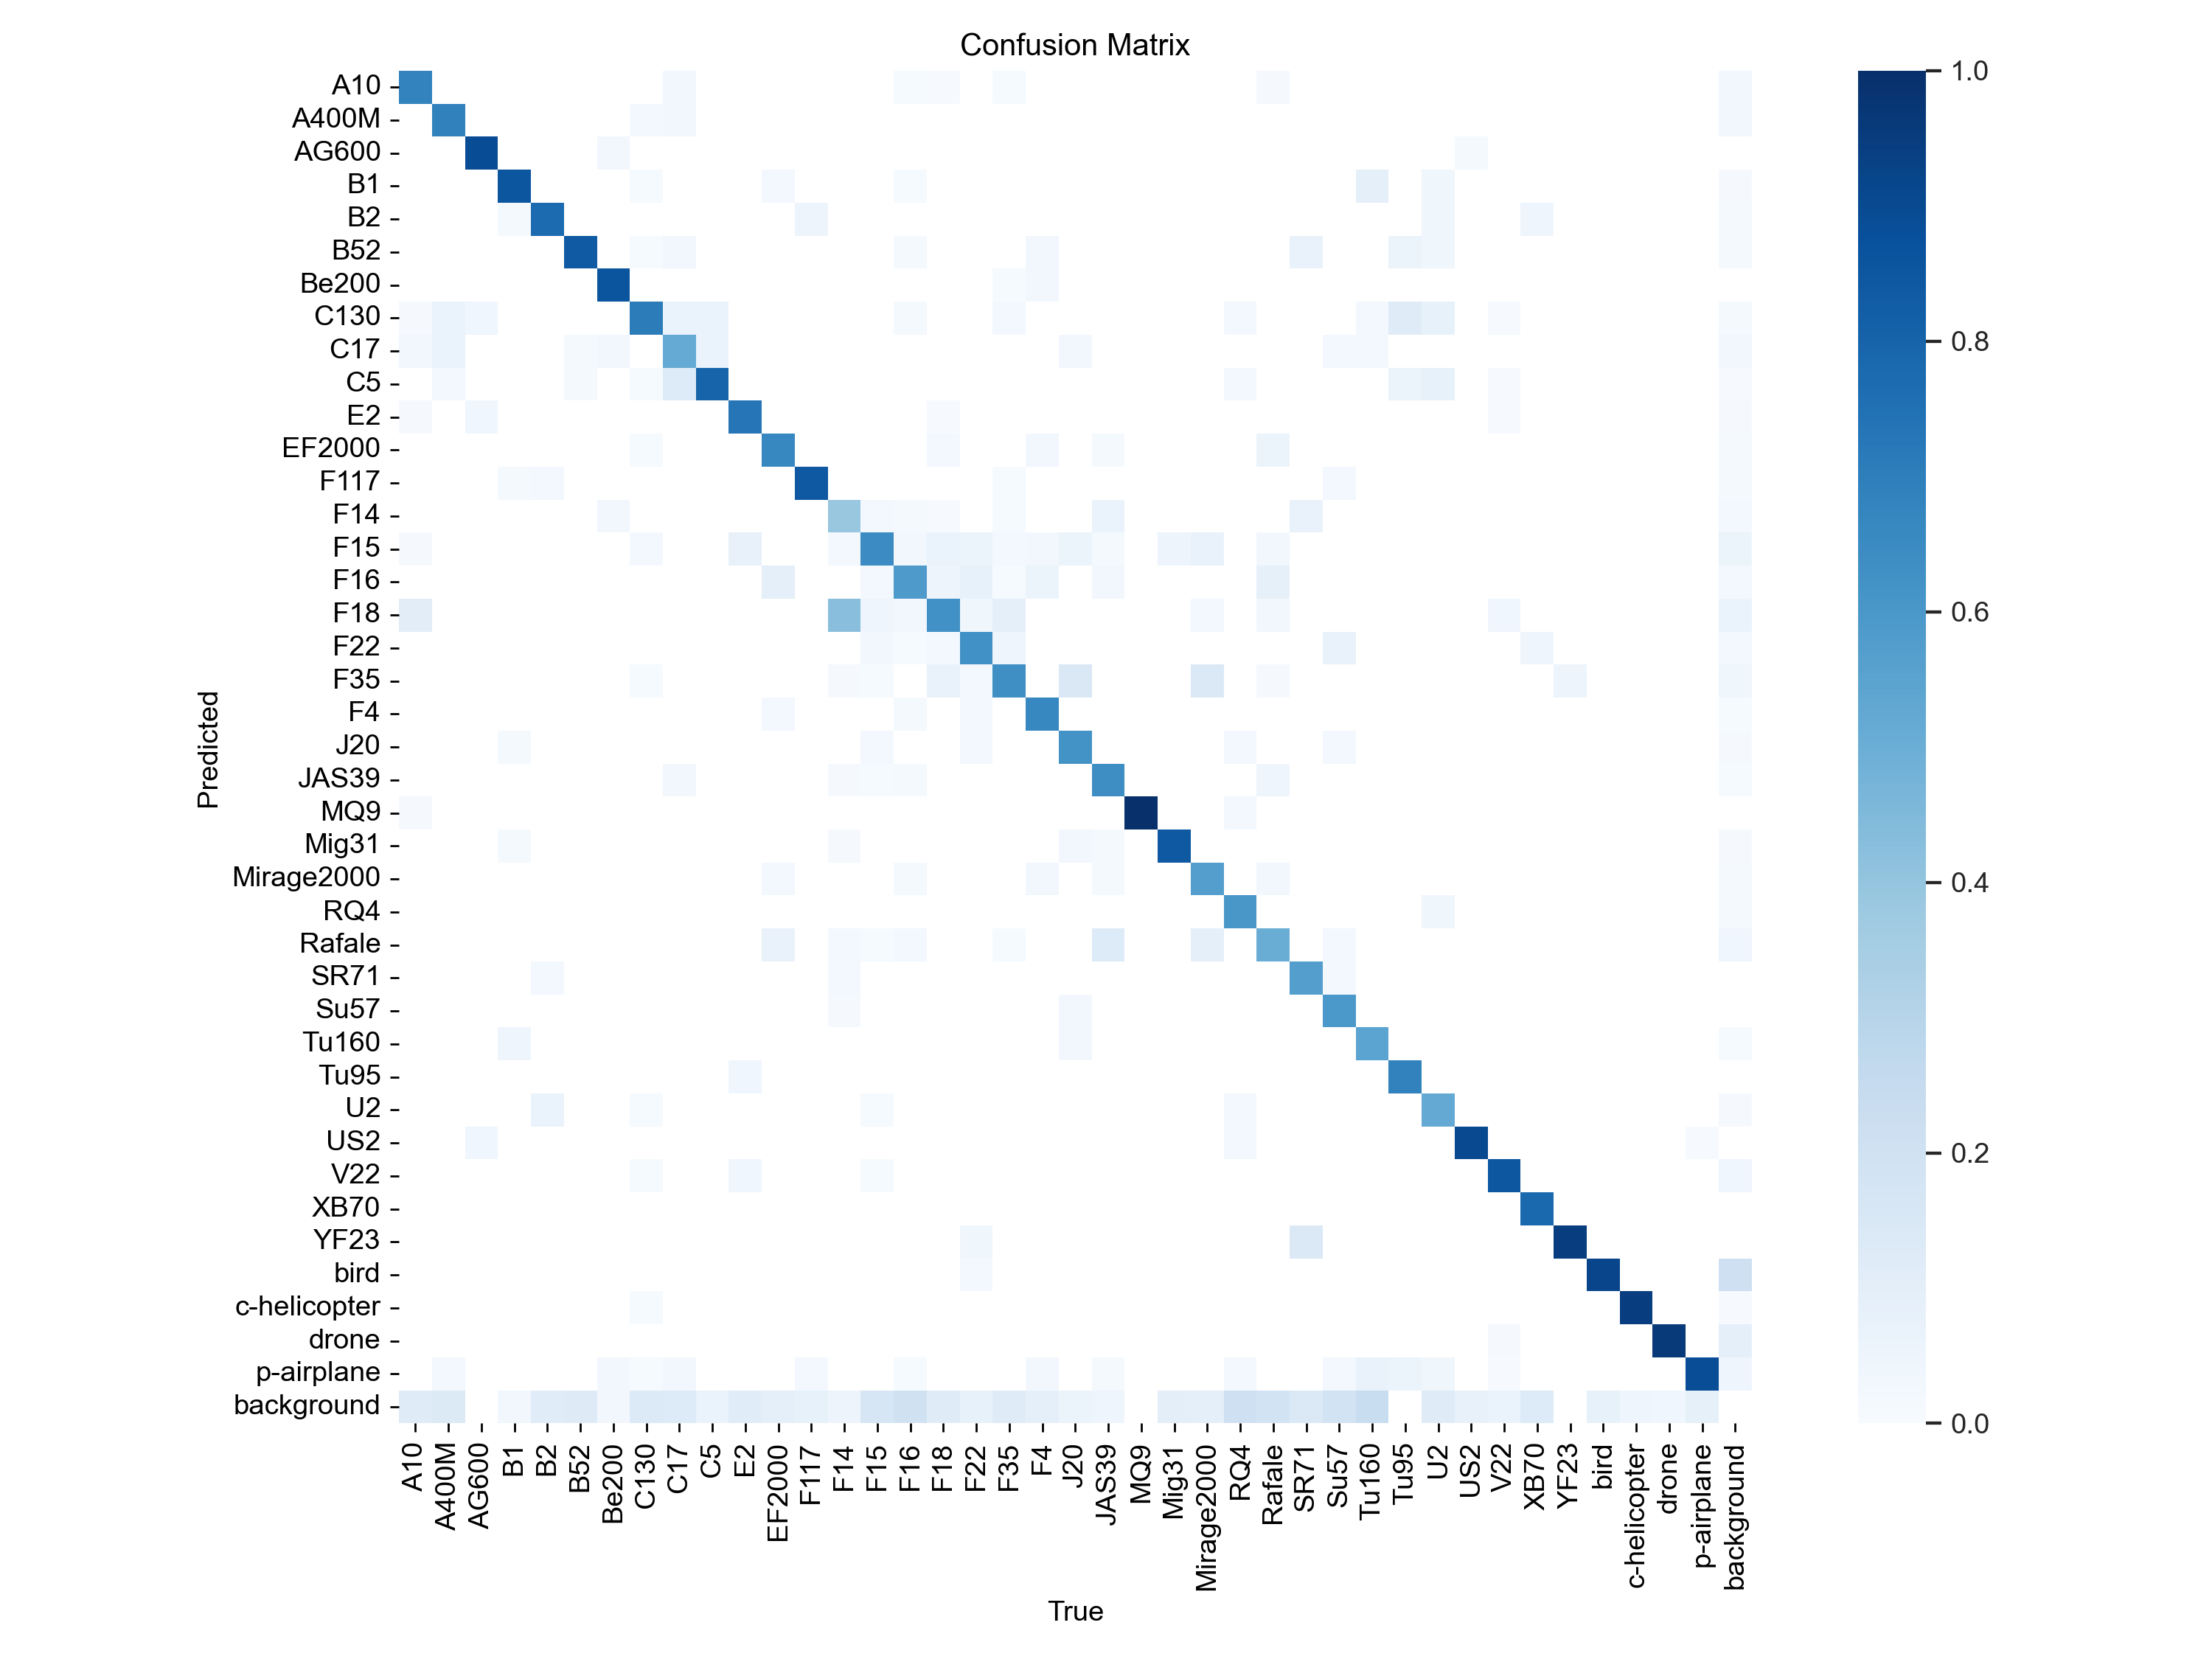
\includegraphics[width=9.5cm,height=7cm]{figures/confusion_matrix.png}}}
    \qquad
    \subfloat[\centering YOLOv8 validation mAP50-95 \label{fig:YOLOv8_mAP50-95_val}]{{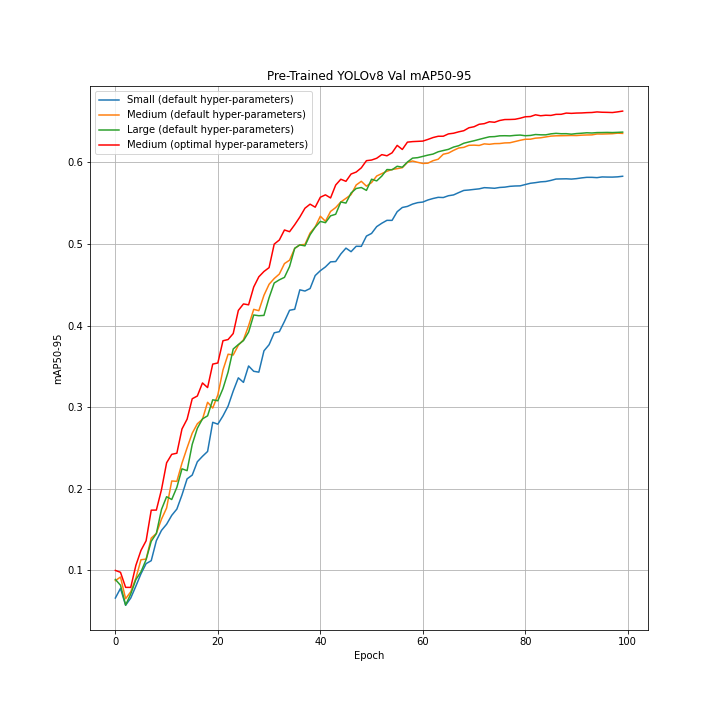
\includegraphics[width=7cm,height=7.9cm]{figures/Pre-Trained YOLOv8 Val mAP50-95.png} }}%
    \caption{YOLOv8 Validation}%
    \label{fig:Model_Evaluation}
\end{figure*}

\section{Experiments and Results}
\subsection{Low Feature Activation Variance Classes}

\begin{figure*}[h]
    \centering
    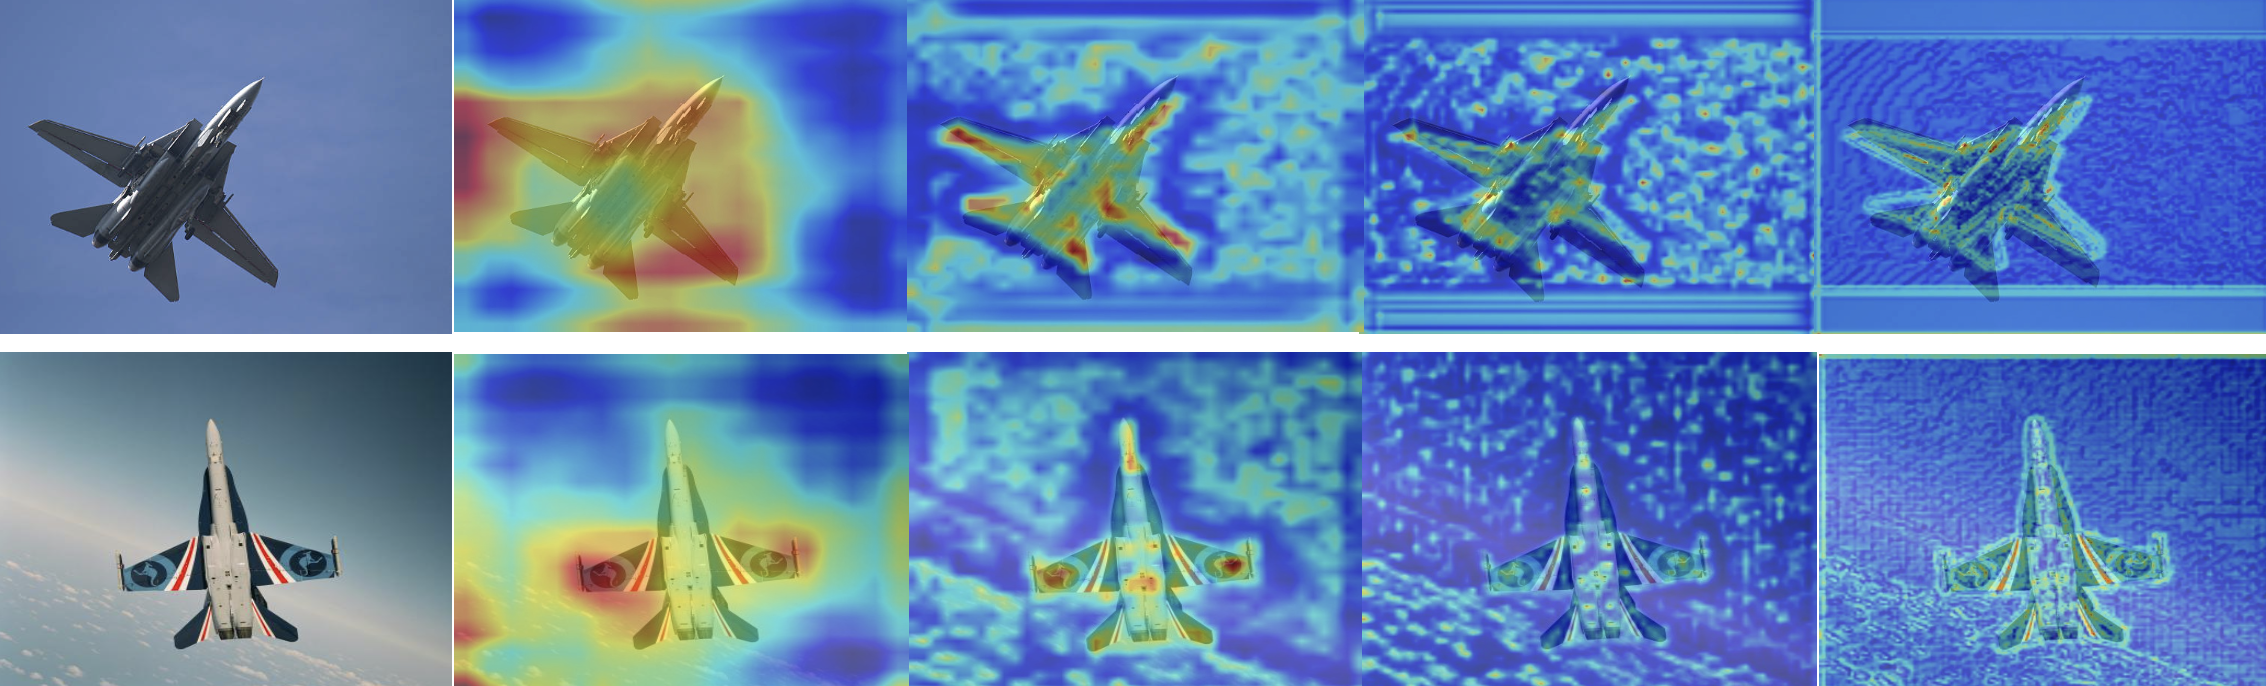
\includegraphics[width=1.0\textwidth]{figures/F14vsF18.png}
    \caption{Feature Activation maps for the F-14 and F-18 fighter jets. From left to right we have the four stages of the model’s
CSPDarkNet53 backbone}
    \label{fig:F14vsF18}
\end{figure*}


One of the primary challenges in object detection is dealing with datasets with low intra-class variance, i.e., multiple classes that look similar to each other compared to the rest of the labels. Take, for example, the F-14 and F-18. Both have similar-looking wing shapes, two rudders, an engine, a cockpit, and weapon systems. In this confusion matrix \ref{fig:Model_Evaluation}, the model is most likely to misclassify an F-14 as an F-18. This type of misclassification typically affects classes in categories with low intra-class variance amongst themselves. Visualizing activation maps \cite{MMYOLOViz} is a technique that helps us understand how the network is processing images and what features and abstractions are being learned. 

Given the nature of a convolutional neural network, generally, the deeper into a network a layer is, the more complex the feature it is learning. YOLOv8 incorporates this idea into its architecture by having repeating modules and multiple detection heads when making its prediction. For our experimentation, we use MMYolo \cite{MMYOLOViz} to create activation maps at different stages of our backbone. We expect to see the different maps showing different levels of granularity for our activations, where the more profound the network activation, the finer and more complex the details are for each class. If our model shows similar feature activations for F-14s and F-18s, we can diagnose this problem as our model shows class confusion.

MMYolo \cite{MMYOLOViz} by Yamaguchi et al. is an open-source toolbox for YOLO series algorithms based on PYTorch. MMYolo can decompose the most popular YOLO algorithms, making them easily customizable and ready for analysis. For our project, we employed MMYolo to first convert the weights from .pt (Pytorch model) to .pth (State dictionary file, i.e., weights, bias, etc.) and second visualize the different activation maps of YOLOv8 during inference. MMYolo allows you to specify model type, weight file, target layer, and channel reduction.

YOLOv8 \ref{fig:YOLOv8_arch} uses CSPDarknet53 \cite{darkNet} as its backbone, a deep neural network that extracts features at multiple resolutions (scales) by progressively downsampling the input image. The feature maps produced at different resolutions contain information about objects at different scales in the image and different levels of detail and abstraction. YOLOv8 can incorporate different feature maps at different scales to learn about object shapes and textures, which helps it achieve high accuracy in most object detection tasks. YOLOv8 backbone consists of four sections, each with a single convolution followed by a c2f module \cite{YOLOv8Website}. The c2f module is a new introduction to CSPDarknet53. The module comprises splits where one end goes through a bottleneck module(Two 3x3 convolutions with residual connections. The bottleneck module output is further split N times where N corresponds to the YOLOv8 model size. These splits are all finally concatenated and passed through one final convolution layer. This final layer is the layer we will get the activations.

This figure \ref{fig:F14vsF18} shows the original F-14 and F-18 images and the activations of the four c2f stages in the network, with each stage being more profound in the network from the second image right. The Activation Map corresponding to the shallowest c2f module shows the broadest activation. This module detects the two wings of the aircraft and determines that this object is a plane. The second activation map corresponds to the second c2f module in our backbone. It shows strong activations at different components of the aircraft, such as locating the wings, body, cockpit, and weapons system onboard. This layer determines what kind of aircraft is being presented in the image by highlighting these features. The third activation map is now showing and is starting to dive into the individual textures of the components of the aircraft, presumably checking for minute differences in parts. Finally, the model's final c2f module activates extremely fine-grained details in the images. Both the F-14 and F-18 have an outline around the plane, leading the model to detect the overall shape of the aircraft. Similar feature activation maps generally mean the model will classify objects the same. The F-14 and F-18 images' features activate the same across multiple layers, explaining why the model is experiencing class confusion for these two classes.

\subsection{Initial Model Results}

[TODO] ADD HYPOTHESES

To highlight our results, we addressed three challenging conditions: (1) detecting and classifying extremely small objects, (2) identifying flying objects that blend into their background, and (3) classifying multiple different types of flying objects. We examined the performance of our initial model, trained on the initial dataset \cite{InitialDataset}, against these challenges. This is demonstrated in Figure \ref{fig:Initial Model Performance}, which features four images that represent the bird, drone, p-airplane, and V22 classes.

The first of the four images showcases the model's ability to identify distant birds. In the second image, the model was put to the test against a very small drone that occupied only .026\% of the image size while also blending in with its background. The model still resulted in the correct detection and classification of the drone. The third image shows the model's ability to identify a minute p-airplane of size 0.063\% of the image, which is also blended into its surroundings. Finally, the fourth image features a V22 aircraft, which is an underrepresented class and accounts for only 3.57\% of the entire dataset. A V22 can easily be mistaken as a drone due to its vertical propeller positioning. Despite these two characteristics and only taking up 0.14\% of the entire image, the image exhibits the model's ability to still identify the V22 with impressive accuracy, achieving a confidence score of 0.83.

Despite the visual similarities between the birds, drone, and p-airplane in these images, our model successfully classified them with adequate confidence. These results illustrate our model's ability to overcome our identified challenges associated with object detection in real-world conditions, and also demonstrate our success in creating a solution that effectively tackles these challenges. Overall, it does very well at distinguishing various types of flying objects despite the need to account for multiple different classes of aircraft.

\begin{figure}[h]
    \centering
    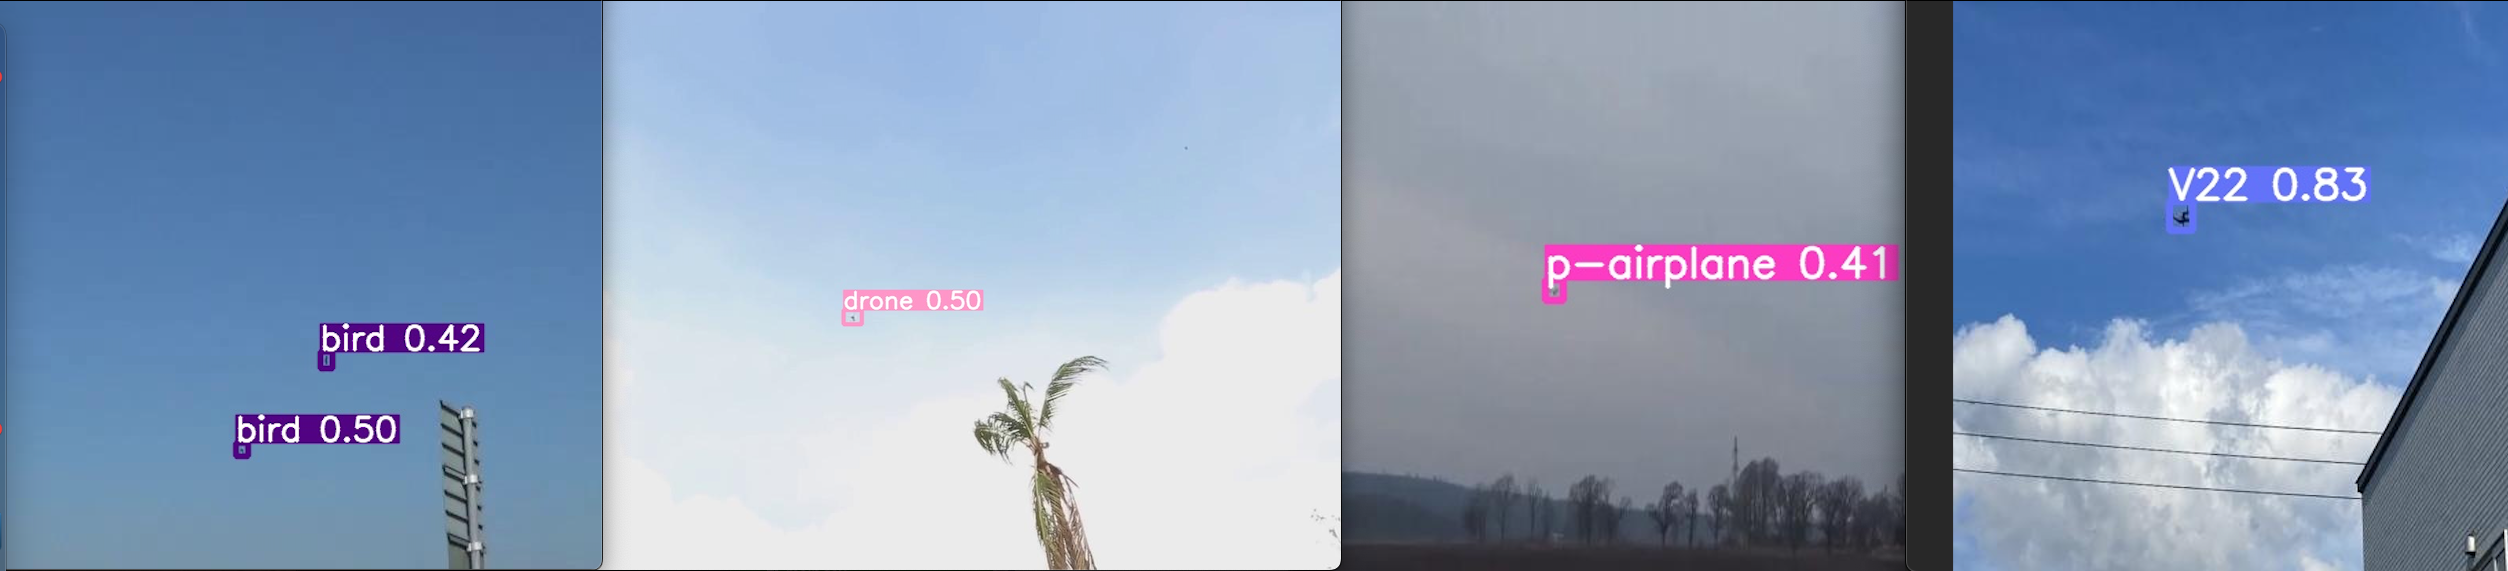
\includegraphics[width=0.5\textwidth]{figures/original_model.png}
    \caption{Initial Model Performance \cite{InitialDataset}}
    \label{fig:Initial Model Performance}
\end{figure}

\subsection{Transfer Learning Results}

[TODO] ADD HYPOTHESES

After applying transfer learning to the dataset with smaller objects \cite{TransferDataset}, the results indicate that our model is a solid foundation for transfer learning. This dataset was selected to focus on our challenge of detecting and classifying extremely small objects in appearance. As a reminder, the bird images were not labeled, making it not possible to train our model to identify them as a class. Figure \ref{fig:Transfer Model Performance} displays our results, featuring four distinct images that represent the bird, drone, airplane, and helicopter objects.

The first image displays a small, pixelated bird that only takes up 0.02\% of the image. Even with the lack of the bird class in our training process, our model correctly identified that the object was not any of the other available classes, even while allowing a very low confidence threshold of 0.20. The second image contains a drone, which also only took up 0.02\% of its image. This drone is nearly indistinguishable from the background clouds to the human eye, yet our model was still able to classify it with a confidence score of 0.81. The third image includes a small airplane that takes up 0.034\% of pixels, which our model was still able to correctly identify and classify with a high confidence score of 0.85. In the final image, a barely visible helicopter (0.01\% of the image) was correctly classified with a confidence score of 0.73.

Our model performed exceptionally well, even while presented with the challenges of size, varying flying objects, and camouflaged objects that would be difficult for the human eye to identify. These results demonstrate that our model serves as an excellent base for transfer learning, particularly when dealing with small, pixelated objects, blended backgrounds, and distinguishing between drones and other flying objects.

\begin{figure}[h]
    \centering
    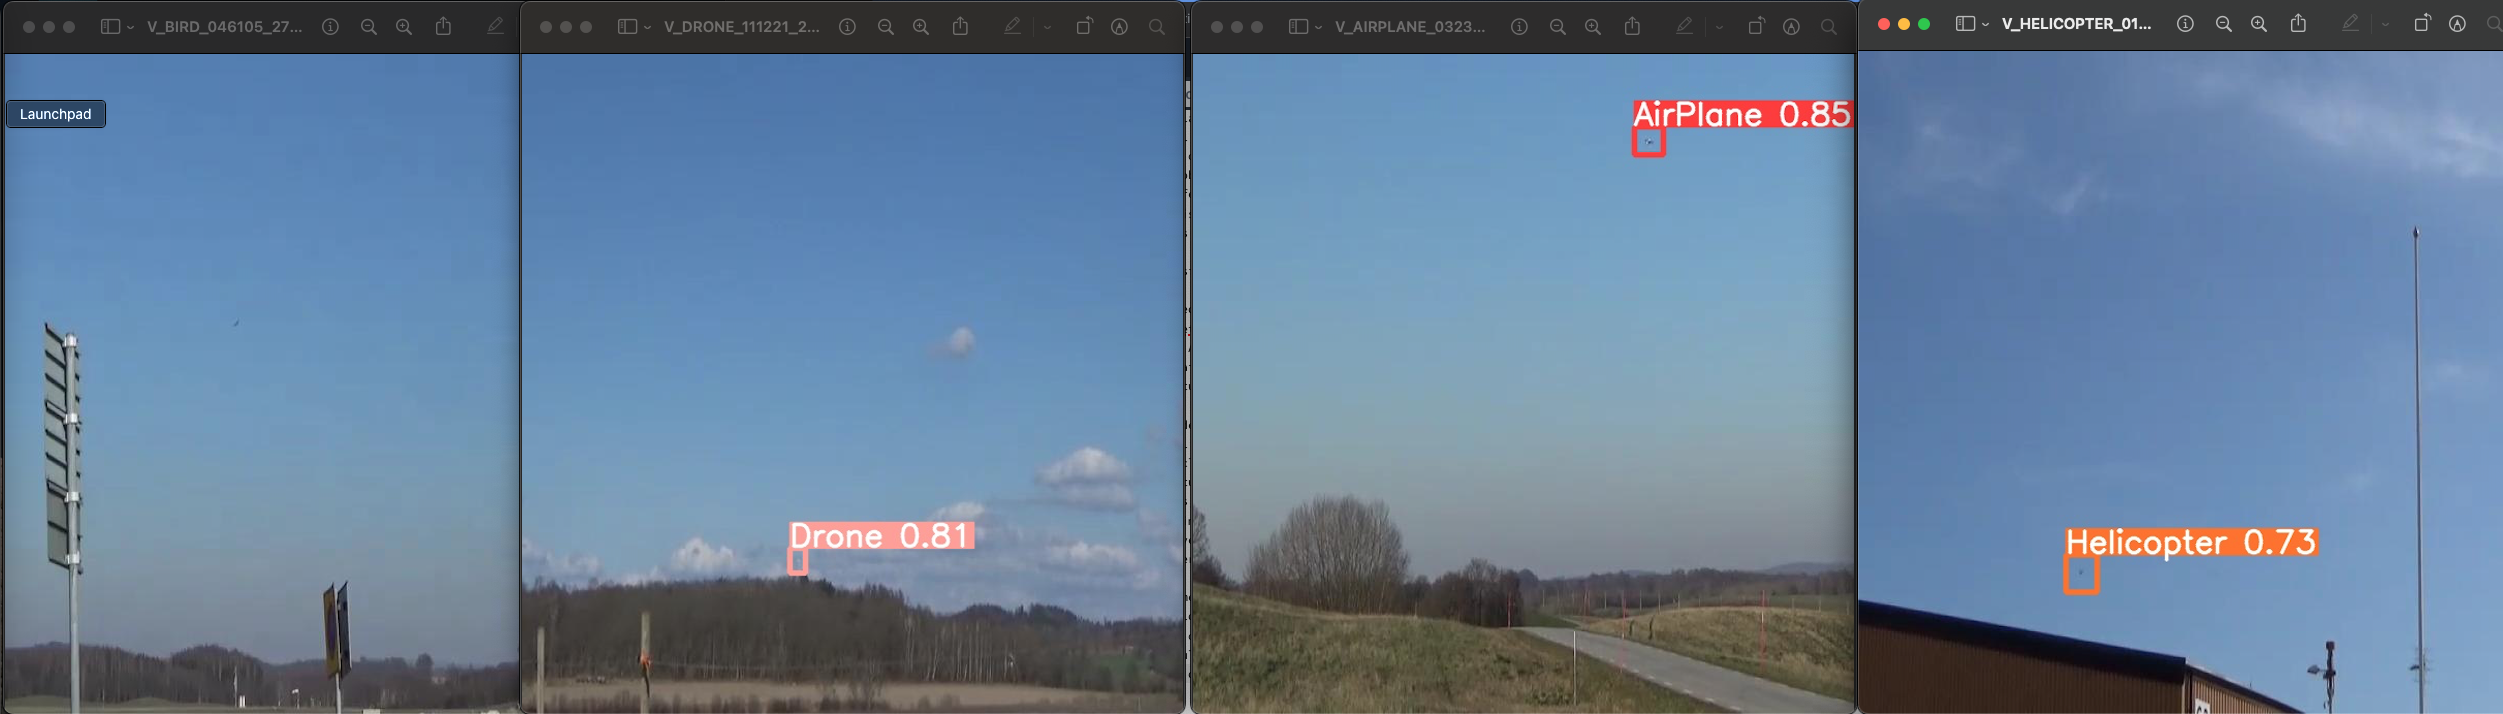
\includegraphics[width=0.5\textwidth]{figures/transfer_model.png}
    \caption{Transfer Model Performance \cite{TransferDataset}}
    \label{fig:Transfer Model Performance}
\end{figure}

%-------------------------------------------------------------------------

\section{Model Architecture}
With the publication of “You Only Look Once: Unified, Real-Time Object Detection” first proposed by Redmon et al.\cite{YOLO_OG} in 2015, one of the most popular object detection algorithms, YOLOv1, was first described as having a “refreshingly simple” approach \cite{CompReview}. At its inception, YOLOv1 could process images at 45 fps, while a variant, fast YOLO, could reach upwards of 155 fps. It also achieved high mAP compared to other object detection algorithms at the time.\\
\indent The main idea of YOLO is to frame the problem of object detection as a one-pass regression problem, YOLOv1 comprises a single neural network, predicting bounding boxes and associated class probability in a single evaluation. The base model of YOLO works by first dividing the input image into an S x S grid where each grid cell (i,j) predicts B bounding boxes, a confidence score for each box and C class probabilities. The final output will be a tensor of shape: S x S x (B x 5 + C).

\subsection{YOLOv1 Overview}
YOLOv1 architecture \ref{fig:YOLOv1Architecture} consists of 24 convolutional layers followed by two fully connected layers. In the paper, the authors took the first 20 convolutional layers from the backbone of the network and, with the addition of an average pooling layer and a single fully connected layer, where it was pre-trained and validated on the ImageNet 2012 dataset. During inference, the final four layers and 2 FC layers are added to the network; all initialized randomly.

\begin{figure}[h]
    \centering
    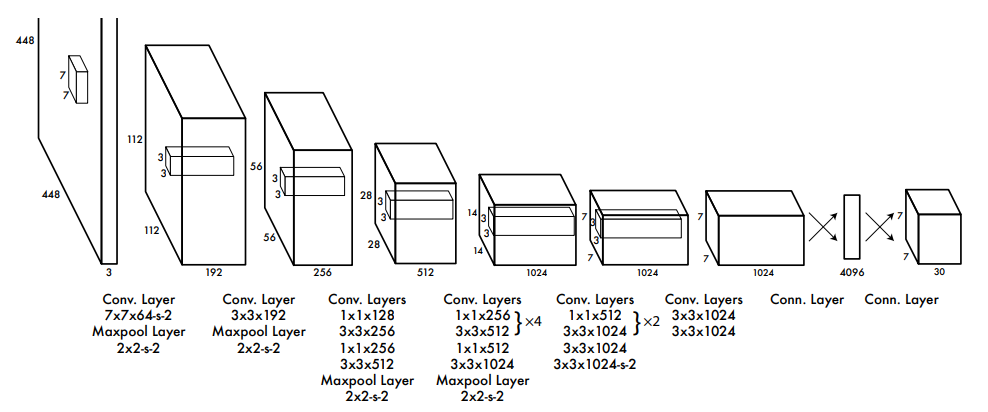
\includegraphics[width=0.4\textwidth]{figures/YOLOv1 Architecture.png}
    \caption{YOLO Architecture \cite{YOLO_OG}}
    \label{fig:YOLOv1Architecture}
\end{figure}

% \begin{figure}[h]
%     \centering
%     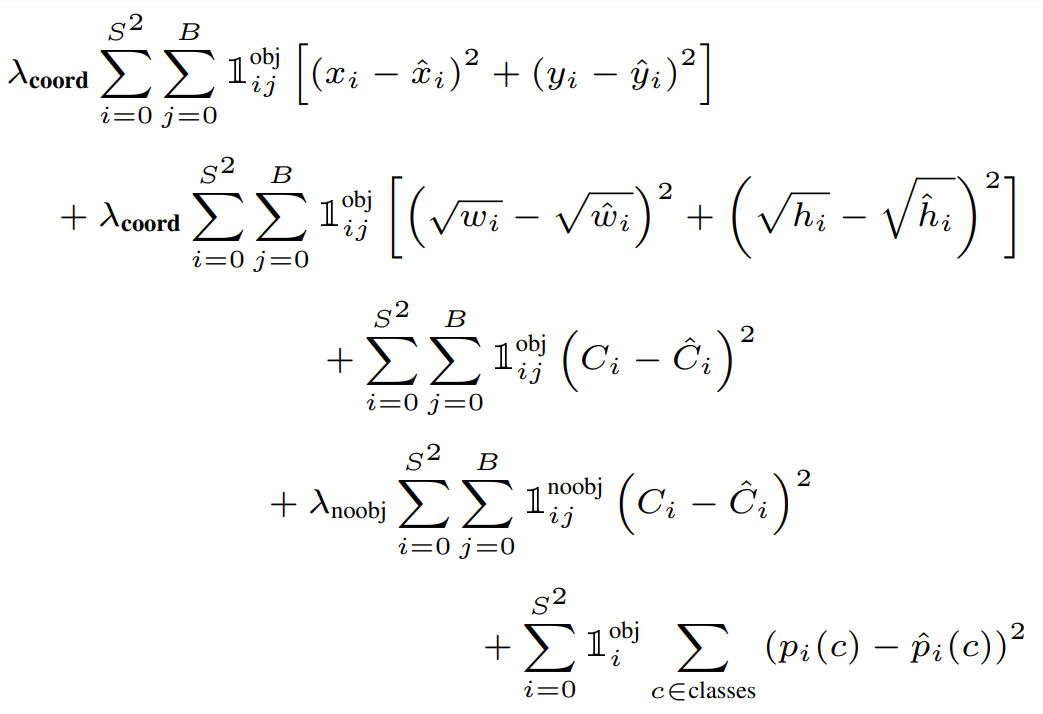
\includegraphics[width=0.4\textwidth]{figures/YOLO_Loss.png}
%     \caption{YOLOv1 Loss function ~\cite{YOLO_OG}}
%     \label{fig:YOLO_Loss}
% \end{figure}\\

YOLOv1 uses stochastic gradient descent as its optimizer; the Loss function is shown here \ref{YOLO_Loss_equation}. The Loss function \ref{YOLO_Loss_equation} comprises two parts, localization loss, and classification loss. The localization loss measures the error between the predicted bounding box coordinates and the ground-truth bounding box. The classification loss measures the error between the predicted class probabilities and the ground truth. The $\lambda_{coord}$ and $\lambda_{noobj}$ are regularization coefficients that regulate the magnitude of the different components, emphasizing object localization and deemphasizing grid cells without objects. 

\begin{multline} \label{YOLO_Loss_equation}
\lambda_{coord}\sum_{i=0}^{S^2}\sum_{j=0}^{B}\mathbbm{1}_{ij}^{obj}\Big[(x_i-\hat{x}_i)^2+(y_i-\hat{y}_i)^2\Big] \\ + \lambda_{coord}\sum_{i=0}^{S^2}\sum_{j=0}^{B}\mathbbm{1}_{ij}^{obj}\Big[(\sqrt{w_i}-\sqrt{\hat{w}_i})^2+(\sqrt{h_i}-\sqrt{\hat{h}_i})^2\Big]\\
+\sum_{i=0}^{S^2}\sum_{j=0}^{B}\mathbbm{1}_{ij}^{obj}(C_i-\hat{C}i)^2\\
+\lambda_{noobj}\sum_{i=0}^{S^2}\sum_{j=0}^{B}\mathbbm{1}_{ij}^{noobj}(C_i-\hat{C}i)^2\\
+\sum_{i=0}^{S^2}\mathbbm{1}_{i}^{obj}\sum_{c\in classes}(p_i(c)-\hat{p}_i(c))^2
\end{multline}

\subsection{YOLOv5 Overview}

YOLOv5 \cite{Drone-Detection-Using-YOLOv5} is an object detection model introduced in 2020 by Ultralytics, the originators of the original YOLOv1 and YOLOv3. YOLOv5 achieves SOTA performance on the COCO benchmark dataset \cite{YOLOv5 doc} while also being fast and efficient to train and deploy. YOLOv5 made several architectural changes, most notably the standardized practice of structuring the model into three components, the backbone, neck, and head.

The backbone of YOLOv5 is Darknet53, a new network architecture that focuses on feature extraction characterized by small filter windows and residual connections. Cross Stage Partial connections enable the architecture to achieve a richer gradient flow while reducing computation as described \cite{cspNET} proposed by Wang et al. 

The neck \cite{YOLOv1->YOLOv8}, as described by Teven et al., of YOLOv5 connects the backbone to the head, whose purpose is to aggregate and refine the features extracted by the backbone, focusing on enhancing the spatial and semantic information across different scales. A Spatial Pyramid Pooling (SPP) \cite{SPP} module removes the fixed-size constraint of the network, which removes the need to warp, augment, or crop images. This is followed by a CSP-Path Aggregation Network \cite{cspNET} module, which incorporates the features learned in the backbone and shortens the information path between lower and higher layers.

YOLOv5’s head consists of three branches, each predicting a different feature scale. In the original publication of the model \cite{YOLOv5Doc}, the creators used three grid cell sizes of 13 x 13, 26 x 26, and 52 x 52, which each grid cell predicting B = 3 bounding boxes. Each head produces bounding boxes, class probabilities, and confidence scores. Finally, the network uses Non-maximum Suppression (NMS) \cite{NMS} to filter out overlapping bounding boxes.

YOLOv5 incorporates anchor boxes, fixed-sized bounding boxes used to predict the location and size of objects within an image. Instead of predicting arbitrary bounding boxes for each object instance, the model predicts the coordinates of the anchor boxes with predefined aspect ratios and scales and adjusts them to fit the object instance.


\begin{figure*}[h]
    \centering
    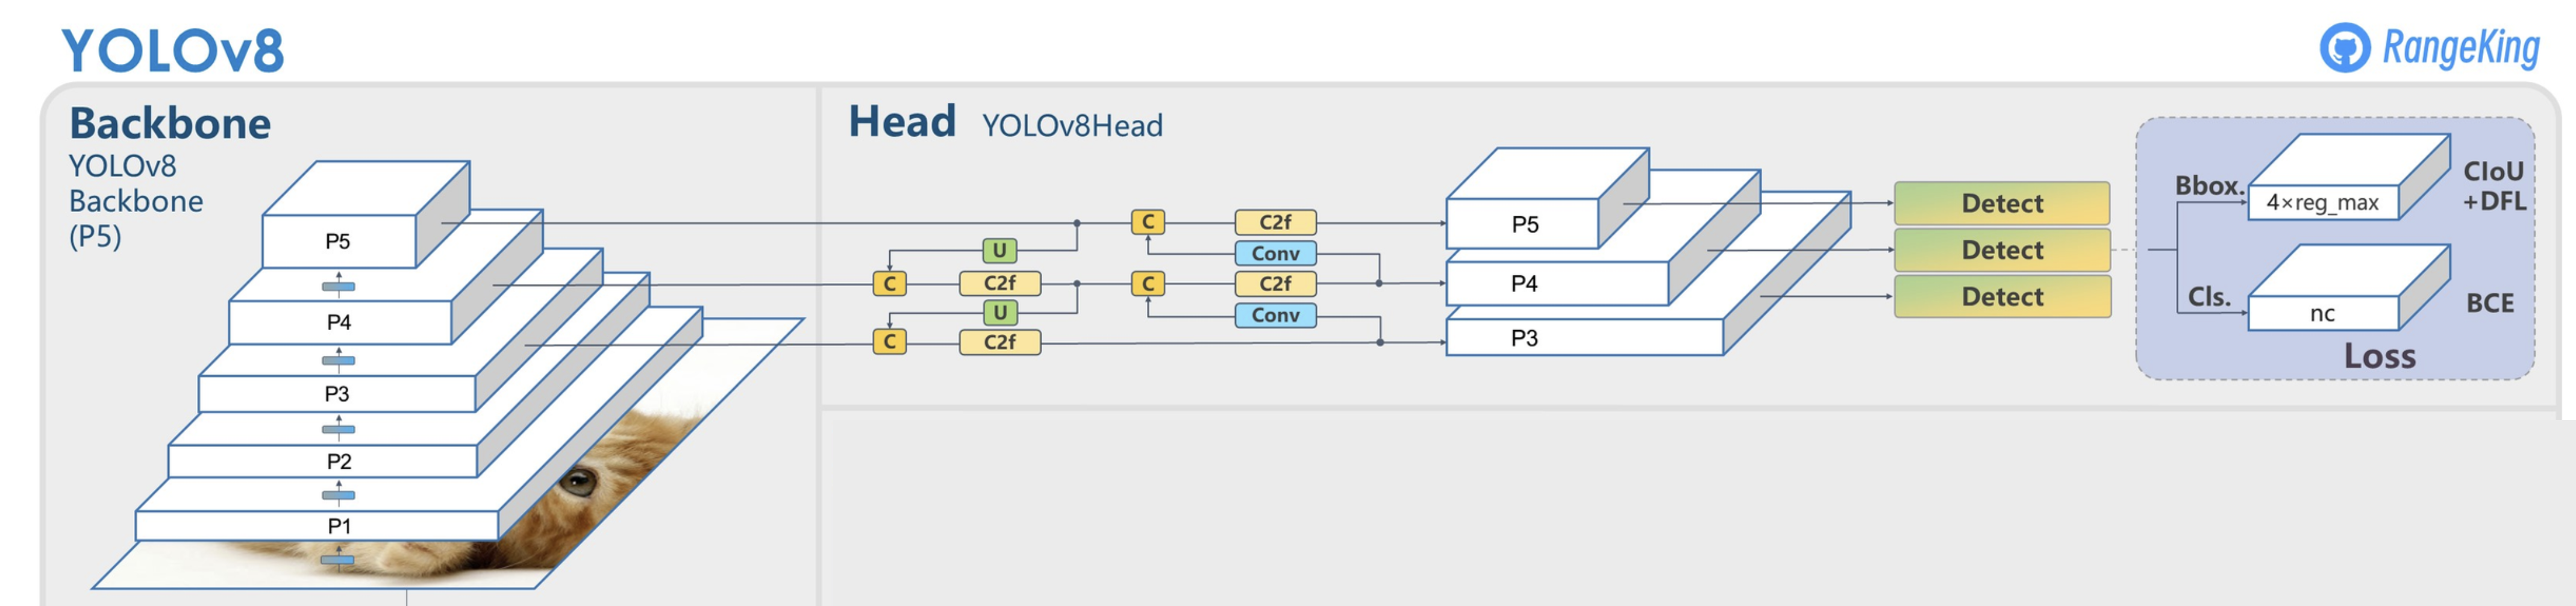
\includegraphics[width=1.0 \textwidth]{figures/YOLOv8_arch.png}
    \caption{YOLOv8 Architecture ~\cite{YOLOv8Website}}
    \label{fig:YOLOv8_arch}
\end{figure*}
\begin{figure}[h]
    \centering
    \subfloat[\centering YOLOs mAP@.50 against RF100 ~\cite{YOLOv8Website} \label{fig:YOLOv8_mAP}]{{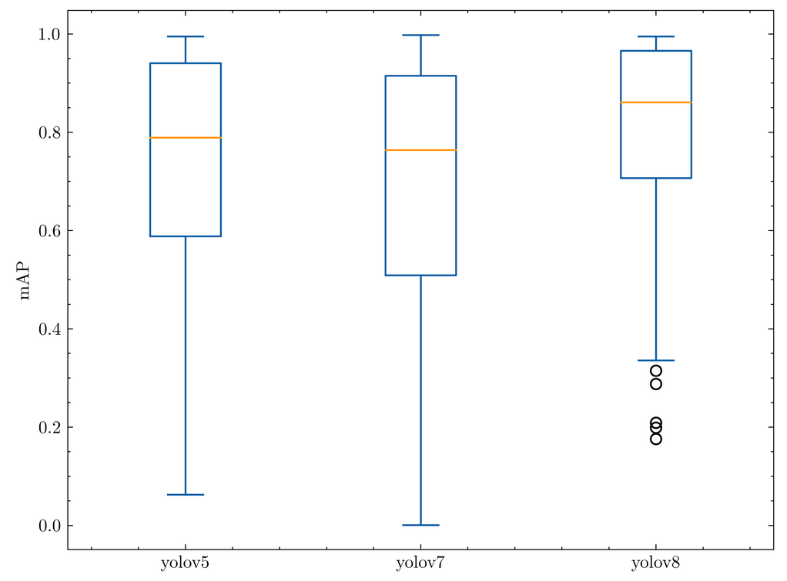
\includegraphics[width=3cm]{figures/YOLOv5_vs_YOLOv8_COMP1.png}}}
    \qquad
    \subfloat[\centering YOLOs average mAP@.50 against RF100 categories \label{fig:YOLOv8_average_mAP_against_cats}]{{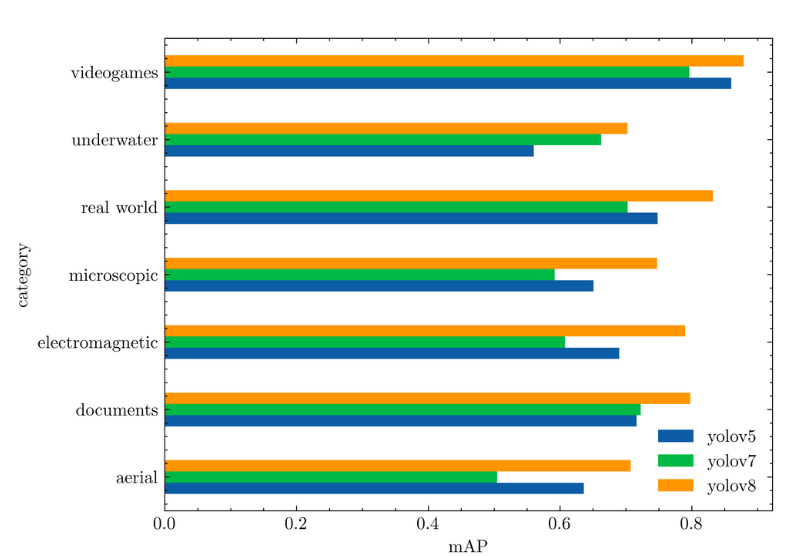
\includegraphics[width=3cm]{figures/YOLOv5_vs_YOLOv8_COMP2.png} }}%
    \caption{YOLOv8 vs Previous Versions}%
    \label{fig:Model_Evaluation2}
\end{figure}

\subsection{YOLOv8 Overview}
YOLOv8 is the latest version of the YOLO object detection model. This latest version has the same architecture as its predecessors \ref{fig:YOLOv8_arch} but it introduces numerous improvements compared to the earlier versions of YOLO such as a new neural network architecture that utilizes both Feature Pyramid Network (FPN) and Path Aggregation Network (PAN) and a new labeling tool that simplifies the annotation process. This labeling tool contains several useful features like auto labeling, labeling shortcuts, and customizable hotkeys. The combination of these features makes it easier to annotate images for training the model.

The FPN works by gradually reducing the spatial resolution of the input image while increasing the number of feature channels. This results in the creation of feature maps that are capable of detecting objects at different scales and resolutions. The PAN architecture, on the other hand, aggregates features from different levels of the network through skip connections. By doing so, the network can better capture features at multiple scales and resolutions, which is crucial for accurately detecting objects of different sizes and shapes ~\cite{CompReview}

\subsection{YOLOv8 vs YOLOv5}
The reason YOLOv8 is being compared to YOLOv5 and not any other version of YOLO is that YOLOv5’s performance and metrics are closer to YOLOv8’s. However, YOLOv8 surpasses YOLOv5 in aspects including a better mAP as seen in Figure \ref{fig:YOLOv8_mAP}. Along with a better mAP, this shows that YOLOv8 has fewer outliers when measured against the RF100 which is a 100-sample dataset from the Roboflow universe which is a repository of 100,000 datasets. We also witness YOLOv8 outperforming YOLOv5 for each RF100 category. From the Figure \ref{fig:YOLOv8_average_mAP_against_cats} we can see that YOLOv8 produces similar or even better results compared to YOLOv5 ~\cite{YOLOv8Website}.

As mentioned previously, YOLOv8 uses a new architecture that combines both FAN and PAN modules. FPN is used to generate feature maps at multiple scales and resolutions, while PAN is used to aggregate features from different levels of the network to improve accuracy. The results of the combined FAN and PAN modules are better than YOLOv5 which uses a modified version of CSPDarknet architecture. This modified version of CSPDarknet is based off the cross-stage partial connections (CSP), which improves the flow of information between different parts of the network.

Another difference the two models have is their training data. YOLOv8 was trained on a larger and more diverse dataset compared to YOLOv5. YOLOv8 was trained on a blend of the COCO dataset and several other datasets, while YOLOv5 was trained primarily on the COCO dataset. Because of that, YOLOv8 has a better performance on a wider range of images.

YOLOv8 includes a new labeling tool called RoboFlow Annotate which is used for image annotation and object detection tasks in computer vision. RoboFlow Annotate makes it easier to annotate images for training the model and includes several features such as auto labeling, labeling shortcuts, and customizable hotkeys. In contrast, YOLOv5 uses a different labeling tool called LabelImg. LabelImg is an open-source graphical image annotation tool that allows its users to draw bounding boxes around objects of interest in an image, and then export the annotations in the YOLO format for training the model.

YOLOv8 includes more advanced post-processing techniques than YOLOv5, which are a set of algorithms applied to the predicted bounding boxes and objectiveness scores generated by the neural network. These techniques help to refine the detection results, remove redundant detections, and improve the overall accuracy of the predictions. YOLOv8 uses Soft-NMS which is a variant of the NMS technique used in YOLOv5. Soft-NMS applies a soft threshold to the overlapping bounding boxes instead of discarding them outright. Whereas NMS removes the overlapping bounding boxes and keeps only the ones with the highest objectiveness score.

Output heads refer to the final layers of a neural network that predict the locations and classes of objects in an image. In YOLO architecture there are typically several output heads that are responsible for predicting different aspects of the detected objects, such as the bounding box coordinates, class probabilities, and objectiveness scores. These output heads are typically connected to the last few layers of the neural network and are trained to output a set of values that can be used to localize and classify objects in an image. The number and type of output heads used can vary depending on the specific object detection algorithm and the requirements of the task at hand. YOLOv5 has 3 output heads while YOLOv8 has 1 output head. YOLOv8 Does not have small, medium, and large anchor boxes rather it uses an anchor free detection mechanism that directly predicts the center of an object instead of the offset from a known anchor box which reduces the number of box predictions, and that speeds up the post processing process.

It is fair to note that YOLOv8 is slightly slower than YOLOv5 when talking about object detection speed. However, YOLOv8 is still able to process images in real-time on modern GPUs.

Both YOLOv5 and YOLOv8 use mosaic augmentation on the training set. Mosaic augmentation is a data augmentation technique that takes four random images from the training set and combines them into a single mosaic image. This image, where each quadrant contains a random crop from one of the four input images, is then inputted into the model ~\cite{MosaicAug}
%---------------------------------------------------------------------

% \begin{figure}[h]
%     \centering
%     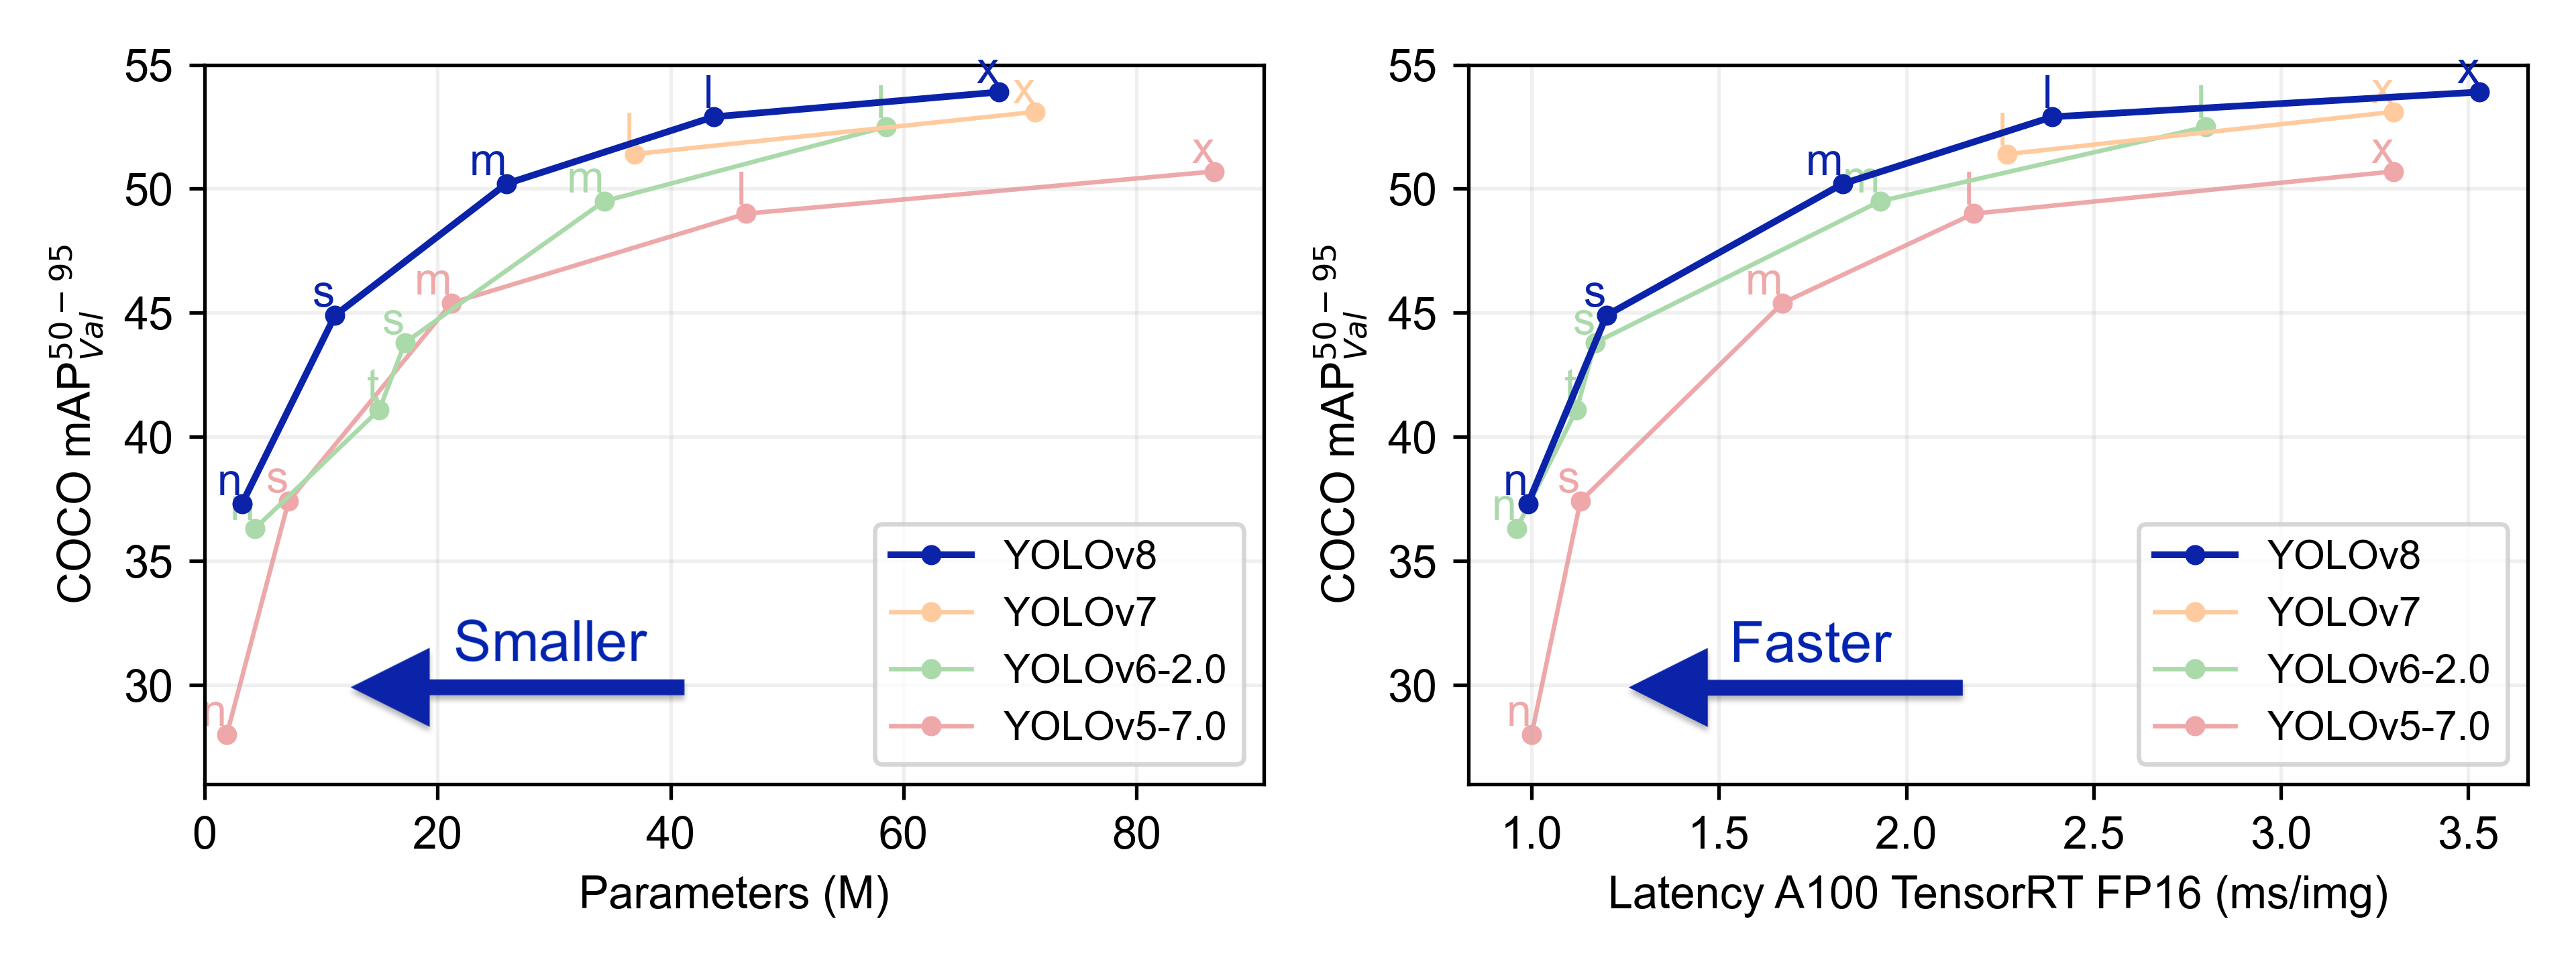
\includegraphics[width=0.45\textwidth]{figures/yolo-comparison-plots.png}
%     \caption{Shows the performance of each YOLO model and its respective versions for mAP50 against a number of parameters and inference speed}
%     \label{fig:my_label}
% \end{figure}

\newpage
\newpage

														 
{\small
\bibliographystyle{ieee_fullname}
\bibliography{egbib}
}

\begin{table*}
\begin{center}			  
\begin{tabular}{|l|c|p{8cm}|}
\hline
Student Name & Contributed Aspects & Details \\
\hline\hline
Team Member 1 & Data Creation and Implementation & Scraped the dataset for this project and trained the CNN of the encoder. Implemented attention mechanism to improve results. \\
Team Member 2 & Implementation and Analysis & Trained the LSTM of the encoder and analyzed the results. Analyzed effect of number of nodes in hidden state.  Implemented Convolutional LSTM. \\
Team Member 3 & Implementation and Analysis & Trained the LSTM of the encoder and analyzed the results. Analyzed effect of number of nodes in hidden state.  Implemented Convolutional LSTM. \\
Team Member 4 & Implementation and Analysis & Trained the LSTM of the encoder and analyzed the results. Analyzed effect of number of nodes in hidden state.  Implemented Convolutional LSTM. \\
\hline
\end{tabular}
\end{center}
\caption{Contributions of team members.}
\label{tab:contributions}
\end{table*}
\end{document}
